\documentclass{article}
\author{
    Epidemiological Modelling Unit,
    \\ School of Public Health and Preventive Medicine,
    \\ Monash University
}
\usepackage{graphicx}
\usepackage{biblatex}
\usepackage{threeparttable}
\usepackage{tabularx}
\usepackage{hyperref}
\usepackage[left=2.5cm,right=2.5cm]{geometry}
% TeX code to create a custom command called \code to allow for the inclusion of inline code
\usepackage{xcolor}
\definecolor{light-gray}{gray}{0.9}  % Define the background colour
\newcommand{\code}[1]{\colorbox{light-gray}{\texttt{#1}}}  % Manual creation of an inline code command

\bibliography{../../references/emu_library}

\title{Modelling methods, Northern Territory application}

\begin{document}

\maketitle
\tableofcontents
\newpage
% This file describes the general structure of some of our tb_dynamics models.

\section{Model Structure}

\subsection{General features}

We use a deterministic compartmental model including six types of compartments that represent 
different states of infection and disease. The model uses the same conceptual approach and similar 
assumptions to previously published models \cite{trauer-2017, ragonnet-2019, ragonnet-2021, ragonnet-2022}. 
Here we describe the model structure without treatment compartment and related factors. 
\newline
A susceptible compartment (S) is used to represent individuals who have 
never been infected with \emph{Mycobacterium tuberculosis (M.tb)}. Latent TB infection (LTBI) is modelled 
using two successive compartments: early latent (E) and late latent (L) to capture the declining risk of 
disease progression over time from infection \cite{ragonnet-2017}. The active disease compartment (I) represents 
individuals who have progressed to the active stage of TB disease. Diseased individuals who recover 
through self-cure progress directly to the recovered compartment (R).
\newline
Non-TB-related mortality is modelled by applying death rates to all model compartments. In addition, 
disease-specific mortality is implemented by applying increased mortality rates to the active disease 
compartments (I).
\newline
Reinfection occurs in the model in two different ways. First, latently infected individuals may be 
reinfected, with this process modelled using a flow from the late latent (L) to the early latent 
compartment (E). Second, individuals who have recovered from TB disease may be reinfected and 
return to the early latent compartment. The structure of our model allows for differential risk of 
infection for the currently and previously infected individuals, compared to the infection-naive 
individuals.
\begin{figure}[!htp]
    \vspace*{-1cm}
    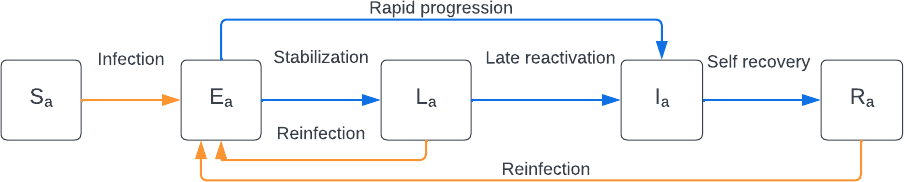
\includegraphics[width=\textwidth,height=\textheight,keepaspectratio]{images/model.png}
    \caption{Illustration of the model structure. 
    Boxes represent the different compartments types: susceptible (S), early latent (E), late latent (L), infectious (I), and recovered (R).
    The subscript indicates that compartments are stratified by age (a).}
    \label{fig:model}
\end{figure}

\subsection{Stratification by age}
The model is stratified using five categories: 0-4, 5-14, 15-34, 35-49 and 50+ years old. We assume 
heterogeneous mixing by age using an age-specific contact rate matrix. Since no local estimates of 
contact patterns by age were available for the Marshall Islands, we used a contact survey conducted in 
the Fijian population and adjusted the estimates to account for age distribution differences between
the two countries.



\begin{figure}[ht]
    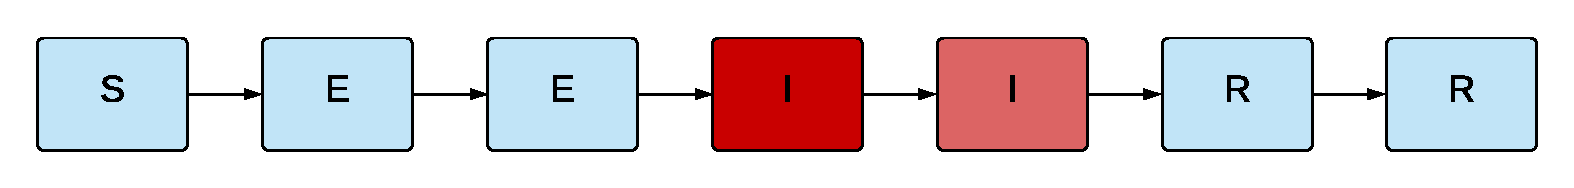
\includegraphics[width=\textwidth]{../../tex_descriptions/models/sm_sir/sm_sir_seir.pdf}
    \caption{Unstratified compartmental model structure. S = susceptible, E = exposed, I = active, R = recovered/removed. Depth of pink/red shading indicates the infectiousness of the compartment.}
    \label{fig:seeiir}
\end{figure}

\subsection{Model stratification}
% Note that this will vary for every application, so will need to be edited - not sure of how best to manage this:
All compartments of the base compartmental structure were stratified by age, location and organ status:\linebreak
Age
\begin{itemize}
    \item Zero to 14 years
    \item 15 to 24 years
    \item 25 to 49 years
    \item 50 to 69 years
    \item 70 years and above
\end{itemize}
Location
\begin{itemize}
    \item South Tarawa
    \item Other location
\end{itemize}
Organ status
\begin{itemize}
    \item Pulmonary smear-posivtive
    \item Pulmonary smear-negative
    \item Extrapulmonary
\end{itemize}

\section{Infectious seed}
The infectious seed value is assigned to the early infectious compartment.
This value is subtracted from the total modelled population and assigned to the susceptible compartment, while all other compartments are assigned a starting value of zero.
This process is undertaken before age stratification is applied,
with the stratification process then splitting these values proportionately according to the starting age distribution of the population.

\section{Clinical stratification} \label{clin}
% Note that this file describes only one implementation of the clinical stratification possible in the sm_sir code
The ``clinical" stratification acts by replicating each of the two age-stratified sequential compartments representing infectious COVID-19 into three categories.
The three clinical categories are:
\begin{enumerate}
    \item Asymptomatic persons
    \item Symptomatic persons who are never notified as cases
    \item Symptomatic persons who are successfully detected and notified
\end{enumerate}
For each age category, a proportion of new active infections are assumed to remain asymptomatic throughout their infectious period (specified in Table \ref{tab:age_params}).
This proportion remains fixed over time throughout a model run.
It is assumed that asymptomatic persons are never detected and so do not contribute to notifications.
The remaining proportion constitutes the second and third categories, comprising all persons developing symptomatic COVID-19 during their infectious period.
The proportion of these symptomatic persons who progress to the third category varies with time and is described under the section on case detection (Section \ref{cdr}).
\begin{figure}[ht]
    \begin{center}
    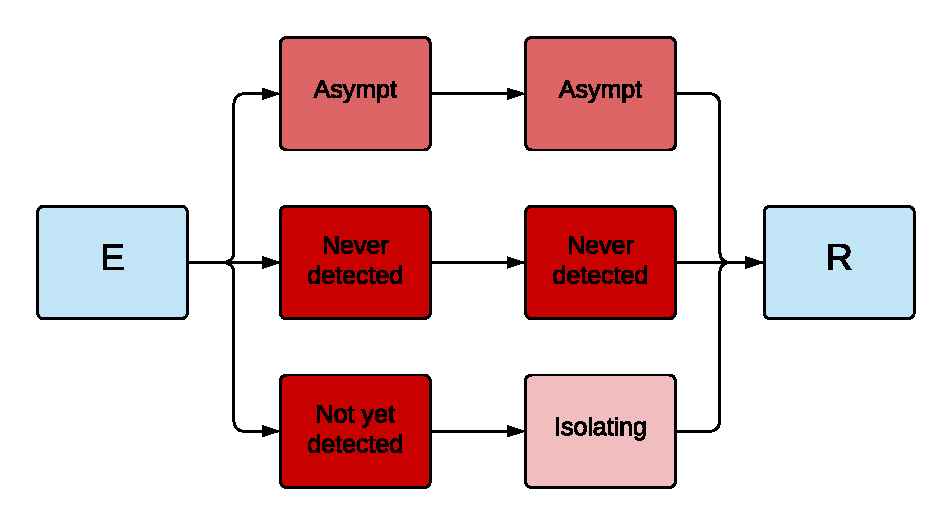
\includegraphics[width=0.7\textwidth]{../../tex_descriptions/models/sm_sir/stratifications/clinical_strat.pdf}
    \end{center}
    \caption{Illustration of the clinical stratification. \small Depth of red shading of compartment qualitatively indicates infectiousness.}
    \label{fig:seeiir}
\end{figure}

The model was stratified by ``strain'' to simulate the emergence of multiple variants of concern (VoC).
This approach explicitly represents multiple competing strains, each with an independent force of infection calculation.
We assumed that VoCs can have different levels of transmissibility, incubation period and disease severity 
(hospitalisation and death risks) compared to the ancestral COVID-19 strain. In addition, VoCs were assumed to escape 
immunity partially for both vaccination- and infection-related immunity. 

We assumed that individuals previously infected with the wild-type strain could only be reinfected with the delta or 
omicron strains. However, such individuals have a reduced risk of infection with these variants compared to 
infection-naive individuals (82\% and 45\% reduction for delta and omicron, respectively) \cite{stein2023}.
We assumed that individuals previously infected with the delta variant could only be reinfected with the omicron variant, 
with an infection risk reduced by 45\% compared to infection-naive individuals \cite{stein2023}. 
The other parameters used to represent strain-specific characteristics are presented in Table \ref{param_table}.

Seeding of each new strain into the model was achieved through the importation of a small number (10 per million population) of new infectious persons with the relevant strain into the model.
The seeding process was implemented over a ten-day period, with the start of this period extracted from the GISAID database for each country \cite{gisaid2023}. 
We considered a strain (either Delta or Omicron) to have emerged when, during a single week in GISAID, at least two cases of that strain were reported, and these cases accounted for at least 1\% of all reported cases during that week.

\subsection{NT strains simulated}
We modelled BA.1, BA.2 and BA.5 as three sequentially emerging strains
in the Northern Territory.
Other strains contributed less to local disease burden 
and so can be considered to be represented by these three strains.
In the counterfactual scenario of early Delta emergence,
the later Omicron strains (BA.2 and BA.5) were not introduced into the model
and parameters for the first strain (BA.1) were adjusted
to reflect the characteristics of Delta.
\section{Vaccination history stratification}
\subsection{General approach}
% Referring to the immunity stratification as the vaccination stratification here, for the NT application
History of vaccination is captured by stratifying all model compartments by vaccination status.
Three vaccination strata are included to represent the following categories:
\begin{itemize}
    \item Persons who have received fewer than two doses of a COVID-19 vaccine (no vaccination or one dose only)
    \item Persons who have received exactly two doses of a COVID-19 vaccine
    \item Persons who have received at least three doses of a COVID-19 vaccine
\end{itemize}
Throughout the analysis period, all the vaccination schedules available in Australia
consisted of a two dose primary course.
The following are not considered in this approach to simulating vaccination:
\begin{itemize}
    \item Any effect of receiving a single dose of vaccine
    \item Waning of vaccine-induced immunity
    \item Any additional effect from receiving additional vaccine doses following the third dose
\end{itemize}
The effect of vaccination on transmission is to partially reduce 
the force of infection for all persons at-risk of infection in the vaccinated stratum.
This applies to both fully susceptible (never previously infected) persons,
as well as recovered persons who are at risk of reinfection.
Emerging variants of concern (VoCs) may escape this immunity, as described in the section on strains.

\subsection{Application to first infection}
The first infection episode with SARS-CoV-2 
is represented through the transition from the susceptible
to the first latent compartment.
The susceptible compartment is not stratified by strain,
because these persons have no infection history.
Therefore, for infection of persons never previously infected,
only the vaccination-induced immunity status is relevant.
The rate of infection for a particular vaccination status is adjusted by the factor:
\[1 - p_{i}\]
Where \(p_{i}\) represents the protection afforded by vaccination stratum \(_{i}\).

\subsection{Application to re-infection}
Persons who have recovered from previous infection episodes 
remain in a compartment that is stratified
according to the last infecting strain.
The recovered compartment is replicated into early and late stages,
which can afford different levels of protection against re-infection.
The rate of reinfection is adjusted by the factor:
\[(1 - p_{i})\times (1 - n_{k,l})\]
Where the additional term \(n_{k,l}\) represents the cross-protection
afforded by past infection with strain \(_{k}\)
against infecting strain \(_{l}\).
In this way, cross-protection can be thought of as the complement
of ``immune escape''/

\subsection{Adjusting age-specific severity parameters for immunity}
We use inputs for the age-specific case fatality rate and the age-specific hospitalisation rate from Nyberg et al., 
which provides estimates of these quantities in a population that already had substantial vaccine-induced immunity.
We therefore adjust these quantities for pre-existing immunity, to account for protection against death and hospitalisation.
We apply the following method to ensure that after adjusting the parameters for a specific age bracket for immunity,
the average parameter value would be equal to that reported by Nyberg et al. if weights were applied according to the
distribution of immunity in the population that was described in this study.
To do this, we estimate the proportion of the population in each of the three modelled immunity categories
in the United Kingdom around the mid-point of the study,
and the protection afforded by each of the immunity classes (see Table \ref{tab:immunity_weighting}).


\begin{table}
    \begin{threeparttable}
    \begin{tabularx}{\textwidth}{| X | X | X | X |}
        \hline
        \textbf{Immunity category} & \textbf{Proportion of population} \tnote{a} & 
        \textbf{Protection against hospitalisation} \tnote{b} & 
        \textbf{Protection against death} \tnote{b} \\
        \hline
        No immunity, unvaccinated & 0.312 & 0 & 0 \\
        \hline
        Low immunity, vaccinated with two doses & 0.302 & 0.5 & 0.8 \\
        \hline
        High immunity, vaccinated with three doses & 0.386 & 0.85 & 0.9 \\
        \hline
	\end{tabularx}
	\caption{Values used to re-weight the severity estimates provided in Nyberg et al. to separate immunity classes.}
	\label{tab:immunity_weighting}
    \begin{tablenotes}
        \item[a] Estimated population distribution as at 16th December 2021 (study mid-point),
        taken from Our World In Data.
        \item[b] Estimated protection against hospitalisation or death following Omicron infection.
    \end{tablenotes}
    \end{threeparttable}
\end{table}

\section{Scaling of contact rates}
The base mixing matrix can be disaggregated into age-specific contacts that occur 
in the following four settings:
\begin{itemize}
    \item Home
    \item Other locations
    \item Work
    \item School
\end{itemize}
The contact rates in each of these settings are scaled as indicated in 
Table \ref{tab:location_scaling}.
The quantity indicated in the Table is considered as a proportion relative to
the baseline value of one.
This quantity is then squared to consider that reductions in mobility will affect
both the potential infector and infectee who will not visit the setting considered.


\begin{table}[h]
    \begin{threeparttable}
    \begin{tabularx}{\textwidth}{| X | X |}
        \hline
        \textbf{Matrix contact setting} & \textbf{Data used to scale contacts} \\
        \hline
        Home & Not scaled \\
        \hline
        Other locations & 
        Flat average of three Google mobility settings time series values
        \begin{itemize}
            \item Grocery and pharmacy
            \item Retail and recreation
            \item Transit stations
        \end{itemize}
        Note that Google provides a mobility metric for parks, 
        which was not used because of the dramatic seasonal variation of this indicator
        in the NT.
        \\
        \hline
        Work & Direct scaling according to the Google mobility workplace time series value \\
        \hline
        School & Mobility not scaled because schools only briefly closed in the NT \\
        \hline
	\end{tabularx}
	\caption{Scaling of mobility values by matrix setting.}
	\label{tab:location_scaling}
    \end{threeparttable}
\end{table}

\section{Calculation of outputs}

\subsection{Incidence}
Incidence is calculated as any transitions into the early active compartment (\textit{``I"}).

\subsection{Hospital occupancy}
Hospitalisation numbers are not reported in the case of Sri Lanka, because the approach to hospitalisation in the country differ considerably from that adopted in the other countries to which the AuTuMN model is applied. Therefore, our approach to simulating hospitalisations is not applicable to Sri Lanka.

\subsection{ICU occupancy}
This is calculated as all persons in the late active compartment in clinical stratum 5.

\subsection{Seropositive proportion}
This is calculated as the proportion of the population in the recovered (\textit{``R"}) compartment. Although very similar numerically to the attack rate, persons who died of COVID-19 are not included in the denominator.

\subsection{COVID-19-related mortality}
This is calculated as all transitions representing death, exiting the model. This is implemented as depletion of the late active compartment.

\subsection{Notifications}
Local case notifications are calculated as transitions from the early to the late active compartment for clinical strata 3 to 5.

\section{Parameters}
\subsection{Age-specific parameters}
Age-structured parameters are presented in Table \ref{tab:age_params}.

\begin{table}
    \begin{threeparttable}
    \begin{tabularx}{\textwidth}{| X | X | X | X | X |}
        \hline
        \textbf{Age group} (years) & \textbf{Clinical fraction} \tnote{a} & 
        \textbf{Relative susceptibility to infection} & \textbf{Case fatality rate} & 
        \textbf{Proportion of symptomatic patients hospitalised} \\
        \hline
        0 to 9   & 0.533 & 0.36 & $5\times10^{-5}$   & 0.011 \\
        \hline
        10 to 19 & 0.533 & 0.36 & $1\times10^{-5}$   & 0.0038 \\
        \hline
        20 to 29 & 0.679 & 1    & $2\times10^{-5}$   & 0.006 \\
        \hline
        30 to 39 & 0.679 & 1    & $5\times10^{-5}$   & 0.0066 \\
        \hline
        40 to 49 & 0.679 & 1    & $1\times10^{-4}$   & 0.0059 \\
        \hline
        50 to 59 & 0.679 & 1    & $5\times10^{-4}$   & 0.0077 \\
        \hline
        60 to 69 & 0.803 & 1    & $2\times10^{-3}$   & 0.0139 \\
        \hline
        70 to 79 & 0.803 & 1.41 & $8.3\times10^{-3}$ \tnote{b} & 0.0357 \tnote{b} \\
        \hline
        80 and above & 0.803 & 1.41 & $5.12\times10^{-2}$ \tnote{b} & 0.111 \tnote{b} \\
        \hline
        Justification and source & 
        Table 1 of systematic review and meta-analysis with appropriate accounting for testing during the pre-symptomatic period\cite{sah-2021}. & 
        Conversion of odds ratios presented in Table S15 of Zhang et al. 2020 to relative risks using data presented in Table S14 of the same study \cite{zhang-2020-a}. &
        Table S2 from Supplemental Materials to Nyberg et al. for ``Hospital admission up to 14 days after positive test''. &  % FIXME: Reference corrupted
        Table S2 from Supplemental Materials to Nyberg et al. for ``Death within 28 days after positive test''. \\  % FIXME: Reference corrupted
        \hline
	\end{tabularx}
	\caption{\textbf{Values used to estimate age-specific parameters.}
    Note that these base parameter values are then adjusted for immunity considerations.}
	\label{tab:age_params}
    \begin{tablenotes}
        \item[a] Proportion of incident episodes developing symptoms.
        \item[b] Modelled age groups are five year brackets to 75 and above.
        These values are used to calculated weighted value for the modelled 75 and above age bracket.
        The value for the 75 and above age group is calculated as the weighted average of the parameters for the 75 to 79 and the 80 and above age groups.
        The weights applied to each of these two groups is the size of the population in the country of application in each of these brackets.
    \end{tablenotes}
    \end{threeparttable}
\end{table}


\begin{table}[h]
    \begin{tabularx}{\textwidth}{| X | p{2.5cm} | X |}
    \hline
    \textbf{Parameter} & \textbf{Value} & \textbf{Rationale} \\
    \hline
    
ISO3 code for source country for mixing matrix & GBR  & Closest demographic profile to Australia \\ 
\hline
Starting infectious seed & 2.0 persons & Arbitrary \\ 
\hline
Proportion of active period before isolation & 0.333  & Assumed \\ 
\hline
Relative infectiousness of asymptomatic persons per unit time & 0.5  & Assumed \\ 
\hline
Relative infectiousness of isolated cases & 0.2  & Assumed \\ 
\hline
Reduction in transmission risk for boosted & 0.6  & Viral load substantially lower in boosted compared to two dose vaccinated persons \cite{puhach-2022} \\ 
\hline
Reduction in transmission risk for primary course & 0.2  & Half of estimate of 40\% for Delta \cite{eyre-2022, harris-2021} \\ 
\hline
Adjustment to base case fatality rates & 0.15  & Adapted to match local epidemiology \\ 
\hline
BA.1 infection cross protection against BA.5 infection & 0.0  & No immunity from BA.1 is retained through to the BA.5 period \\ 
\hline
BA.2 infection cross protection against BA.1 infection & 1.0  & Immunity from subsequent strains is assumed to completely protect against previous strains \\ 
\hline
BA.5 infection cross protection against BA.1 infection & 1.0  & Immunity from subsequent strains is assumed to completely protect against previous strains \\ 
\hline
BA.5 infection cross protection against BA.2 infection & 1.0  & Immunity from subsequent strains is assumed to completely protect against previous strains \\
    \hline
    \end{tabularx}
	\caption{Epidemiological fixed parameter values.}
    \label{tab:fixed_params}
\end{table}

\begin{table}[h]
    \begin{tabularx}{\textwidth}{| X | p{2.5cm} | X |}
    \hline
    \textbf{Parameter} & \textbf{Value} & \textbf{Rationale} \\
    \hline
    
Disease onset to notification distribution & gamma  & Assumed \\ 
\hline
Mean disease onset to notification & 3.0  & Assumed \\ 
\hline
Onset to notification parameter & 5.0  & Assumed \\ 
\hline
Disease onset to death distribution & gamma  & Assumed \\ 
\hline
Mean disease onset to death & 14.0 days & Assumed \\ 
\hline
Onset to death shape parameter & 5.0  & Assumed \\ 
\hline
Disease onset to hospital admission distribution & gamma  & Assumed \\ 
\hline
Mean disease onset to hospital admission & 5.0 days & Assumed \\ 
\hline
Onset to hospitalisation shape parameter & 5.0  & Assumed \\ 
\hline
Proportion of hospitalised persons admitted to ICU & 0.08  & Assumed \\ 
\hline
Disease onset to ICU admission distribution & gamma  & Assumed \\ 
\hline
Mean disease onset to ICU admission & 2.0 days & Assumed \\ 
\hline
Onset to ICU shape parameter & 5.0  & Assumed \\ 
\hline
Distribution type for hospital stay & gamma  & Assumed \\ 
\hline
Mean hospital stay & 3.0 days & Assumed \\ 
\hline
Shape parameter for hospital stay & 5.0  & Assumed \\ 
\hline
Distribution type for ICU stay & gamma  & Assumed \\ 
\hline
Mean ICU stay & 4.7 days & Assumed \\ 
\hline
Shape parameter for ICU stay & 5.0  & Assumed \\
    \hline
    \end{tabularx}
	\caption{Output-related fixed parameter values.}
    \label{tab:output_params}
\end{table}

\begin{table}[h]
    \begin{tabularx}{\textwidth}{| X | p{2.5cm} | X |}
    \hline
    \textbf{Parameter} & \textbf{Distribution type} & \textbf{Distribution parameters} \\
    \hline
    
Probability of transmission per contact & Uniform & Range: [0.15, 0.4] \\ 
\hline
Infection latent period & Uniform & Range: [2.0, 4.0] \\ 
\hline
Period with active disease & Uniform & Range: [1.0, 5.0] \\ 
\hline
Starting infectious seed & Uniform & Range: [50.0, 300.0] \\ 
\hline
Maximum effect of microdistancing & Uniform & Range: [0.0, 0.6] \\
    \hline
    \end{tabularx}
	\caption{Prior distributions of parameters used in model calibration.}
    \label{tab:priors}
\end{table}

\newpage
\printbibliography

\end{document}
